\documentclass[a4paper,11pt]{article}
\usepackage{graphicx}

\begin{document}

\begin{flushright}

\vspace{1.1cm}

%Put ISR Title
{\bf\Huge Problem Set 3}

\rule{0.25\linewidth}{0.5pt}

\vspace{0.5cm}
%Put Authors
Justin Ely
\linebreak
\newline
%Put Author's affiliations
\footnotesize{AST615 University of Maryland College Park, MD\\}
\vspace{0.5cm}
% Date here below
06 November, 2011
\end{flushright}

\noindent\rule{\linewidth}{1.0pt}
\section*{Problem 1}
\subsection*{a,b,c}
Please see included txt files for the output from the script.  For sections b and c, please refer to Figures 1 and 2 below.  The coordinates for the Lagrange points are given in Table 1 below.


\begin{figure}[h!]
\begin{center}
\includegraphics[scale=.4]{3_1_1_system.pdf}
\caption{Plot showing the system for M1=3,M2=1,separation=1.  Contours show effective potential and vectors show effective acceleration.  Note that large acceleration vectors have been suppressed so as not to crowd plot.  As such, vectors close around the masses will appear as zero.  For higher resolution, please open the included pdf.}
\end{center}
\end{figure}

\begin{figure}[h!]
\begin{center}
\includegraphics[scale=.4]{100_1_1_system.pdf}
\caption{Plot showing the system for M1=100,M2=1,separation=1.  Contours show effective potential and vectors show effective acceleration.  Note that large acceleration vectors have been suppressed so as not to crowd plot.  As such, vectors close around the masses will appear as zero.  For higher resolution, please open the included pdf.}
\end{center}
\end{figure}

\begin{table}[h!]
\begin{center}
\begin{tabular}{|c||c|c|c|c|c|}
\hline
 (3,1,1)&L1&L2&L3&L4&L5\\
\hline
 Plotted& (40.5,50)& (76.5,50) & (18.5,50) & (43,70.5) & (43,28.5)\\
 Computed& (-.38,0)& (1.06,0) & (-1.26,0) & (-.28,.82) & (-.28,-.86)\\
\hline
\hline
 (100,1,1)&L1&L2&L3&L4&L5\\
\hline
 Plotted& (28.5,50)& (74.5,50) & (21.5,50) & (37,70.5) & (37,28.5)\\
 Computed& (-.86,0)& (.98,0) & (-1.14,0) & (-.52,.82) & (-.52,-.86)\\
\hline
\end{tabular}
\end{center}
\caption{Plotted and computed coordinates of the Lagrange points for the two systems.  Plotted coordinates give the (x,y) coordinates of the point in the coordinate grid of the figures.  Computed coordinates give the (x,y) coordinates of the point in the G==1 coordinate system.}
\end{table}


\section*{Problem 2}
\section*{a}
After fitting the data in the file, I find $\alpha_{L}=7.69$ and $\nu_{0}=48.28$ for the Lorentzian profile and $\alpha_{D}=12.15$ and $\nu_{0}=47.667$ for the Gaussian profile.  The error estimate for the Lorentzian fit was $9.83x10^{-4}$ and for the Gaussian fit was $-8.74x10^{-6}$.  We can see from both the smaller error estimate and the profiles plotted below in Figure 3, the Gaussian profile is the much better fit to the data.
\section*{b}
\begin{figure}[!h]
\begin{center}
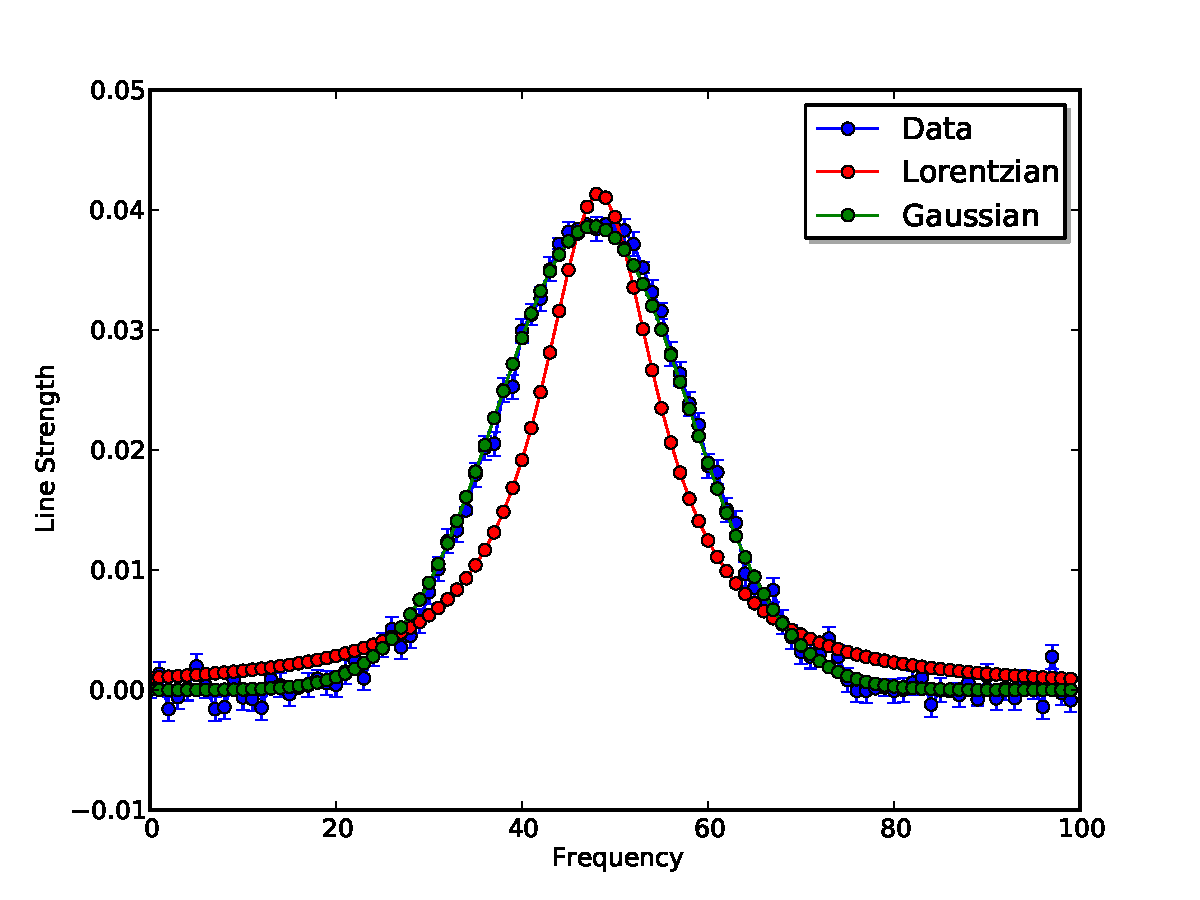
\includegraphics[scale=.7]{fit.pdf}
\caption{Gaussian and Lorentzian fit to ps3.dat.}
\end{center}
\end{figure}

\end{document}
